\documentclass[letterpaper,11pt]{article}

% Soporte para los acentos.
\usepackage[utf8]{inputenc}
\usepackage[T1]{fontenc}    
% Idioma español.
\usepackage[spanish,mexico, es-tabla]{babel}
% Soporte de símbolos adicionales (matemáticas)
\usepackage{multirow}
\usepackage{amsmath}		
\usepackage{amssymb}		
\usepackage{amsthm}
\usepackage{amsfonts}
\usepackage{latexsym}
\usepackage{enumerate}
\usepackage{ragged2e}
\usepackage{graphicx}
\usepackage{hyperref}
\usepackage{caption}
\usepackage{subcaption}
% Modificamos los márgenes del documento.
\usepackage[lmargin=2cm,rmargin=2cm,top=2cm,bottom=2cm]{geometry}

\title{Facultad de Ciencias, UNAM \\ 
       Reconocimiento de patrones y aprendizaje automatizado \\ 
       Tarea 2}
\author{Rubí Rojas Tania Michelle}
\date{\today}

\begin{document}
\maketitle

\begin{enumerate}
    % Ejercicio 1.
    \item Cada una de las líneas en el documento \texttt{tarea2\_docs.txt} lo 
    vamos a considerar como un documento. Realiza la limpieza y preprocesamiento 
    necesarios.

    \textsc{Solución:} Leemos el archivo \textbf{tarea\_docs.txt} línea por 
    línea (ya que cada una de éstas será considerada como un documento) y lo 
    guardamos en un arreglo. Posteriormente, convertimos este arreglo en un 
    \texttt{DataFrame} cuya única columna se llamará \texttt{'text'} y cada una 
    de sus filas contendrá los distintos textos guardados.
    \begin{center}
        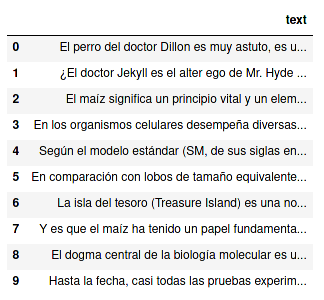
\includegraphics[width=0.4\textwidth]{imagenes/text1.png}
    \end{center}

    Luego, convertimos cada uno de los documentos en vectores usando TFIDF.
    \begin{center}
        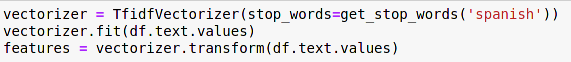
\includegraphics[width=0.65\textwidth]{imagenes/text2.png}
    \end{center}

    Por otro lado, usaremos el algoritmo \textbf{K-means} para agrupar nuestros 
    datos. De esta forma, para encontrar el valor adecuado de $K$ realizamos una 
    gráfica e intenamos hallar el \textit{Elbow Curve}, para lo cual ejecutamos 
    varios \textit{k-means}, incrementamos a $k$ en cada iteración y registramos 
    el valor del SSE.
    \begin{center}
        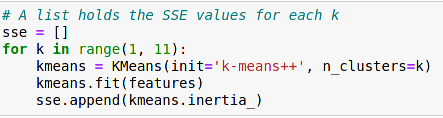
\includegraphics[width=0.45\textwidth]{imagenes/text4.png}
    \end{center}
    \newpage
    \begin{center}
        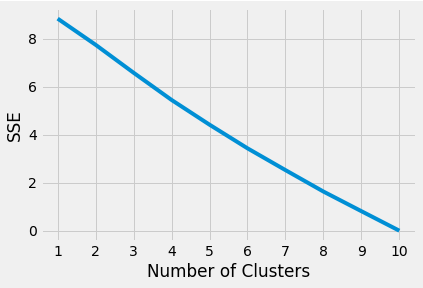
\includegraphics[width=0.35\textwidth]{imagenes/text3.png}
    \end{center}

    donde podemos notar que en $k=5$ se dobla ligeramente la curva. Así, 
    ejecutamos \textbf{K-means} con este valor, realizamos nuestras predicciones 
    y modificamos el \texttt{DataFrame} de tal forma que agregamos la nueva 
    clasificación encontrada.
    \begin{center}
        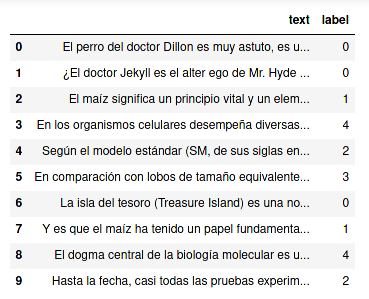
\includegraphics[width=0.45\textwidth]{imagenes/text5.png}
    \end{center}

    Como podemos observar, los textos se clasificaron en $5$ grupos diferentes. 
    Separamos cada texto en un \texttt{DataFrame} distinto para poder visualizar 
    los resultados.
    \begin{figure}[ht]
        \centering
        {{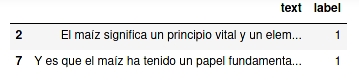
\includegraphics[width=0.4\textwidth]{imagenes/text7.png}}}%
        \qquad
        {{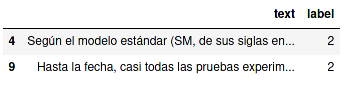
\includegraphics[width=0.4\textwidth]{imagenes/text8.png}}}%
    \end{figure}
    \begin{figure}[ht]
        \centering
        {{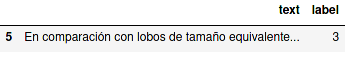
\includegraphics[width=0.4\textwidth]{imagenes/text9.png}}}%
        \qquad
        {{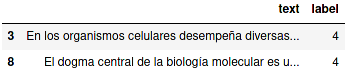
\includegraphics[width=0.4\textwidth]{imagenes/text10.png}}}%
    \end{figure}
    \begin{figure}[ht]
        \centering
        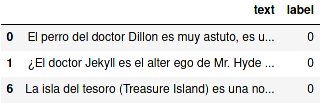
\includegraphics[width=0.4\textwidth]{imagenes/text6.png}
    \end{figure}

    Podemos observar que obtuvimos una muy buena agrupación, pues a mi 
    consideración, sólo agrupó erróneamente un texto (y se encuentra en el 
    grupo $3$).
    
    \newpage
    Contesta las siguientes preguntas:
    \begin{itemize}
        % Ejercicio 1.a
        \item ¿En qué tópicos se pueden dividir?

        \textsc{Solución:} Se puede dividir en $5$ diferentes tópicos:
        \begin{itemize}
            \item Aquellos con la etiqueta $1$, que corresponden a temas 
            relacionados con el maíz en los pueblos indígenas y la cultura 
            mexicana.

            \item Aquellos con la etiqueta $2$, que corresponden a temas 
            relacionados con la física.

            \item Aquel con la etiqueta $3$, que corresponde a la descripción 
            de lobos (el cual debería de estar relacionado con el texto que 
            habla del perro del Doctor Dillon, pues hablan de cosas similares).

            \item Aquellos con la etiqueta $4$, que corresponden a temas de 
            biología molecular.

            \item Aquellos con la etiqueta $0$, que corresponden a descripciones
            de libros (con un integrante erróneo).
        \end{itemize}

        % Ejercicio 1.b
        \item ¿Qué documentos habla de México y su cultura?

        \textsc{Solución:} Los documentos etiquetados con el número $1$.
    \end{itemize}

    % Ejercicio 2.
    \item Descarga el dataset de datos de sonar de la siguiente liga:
    \url{https://archive.ics.uci.edu/ml/machine-learning-databases/undocumented/
    connectionist-bench/sonar/sonar.all-data}

    Mismo que deberás explorar y entender lo que hacen sus atributos. 
    
    Lleva a cabo una clasificación utilizándo la regresión logística de los 
    datos. Luego, efectúa una reducción de dimensión y haz tu clasificación 
    otra vez. La comparación entre las clasificaciones la harás con las 
    métricas que tú elijas. 

    ¿Qué observas y por qué sucede esto?

    \textsc{Solución:} \textbf{sonar.all-data} es un conjunto de datos que 
    describe el sonido (o más bien, el chirrido) del sonar al rebotar sobre 
    diferentes superficies. Las $59$ variables de entrada son la fuerza de los 
    retornos en ángulos diferentes y se encuentran en un rango de $0$ a $1$. La 
    variable $60$ de salida es un string \textbf{M} para Mina y \textbf{R} para 
    Roca.

    El problema es de clasificación binaria, la cual requiere de un modelo para 
    diferenciar rocas de cilindros metálicos.

    Descargamos el conjunto de datos y lo visualizamos.
    \begin{center}
        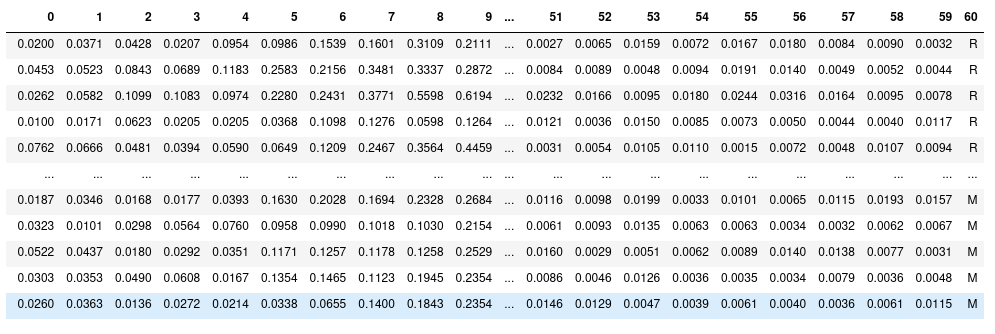
\includegraphics[width=0.8\textwidth]{imagenes/sonar-dataset.png}
    \end{center}

    Veamos si la proporción de los datos en cada clase es equilibrada.
    \begin{center}
        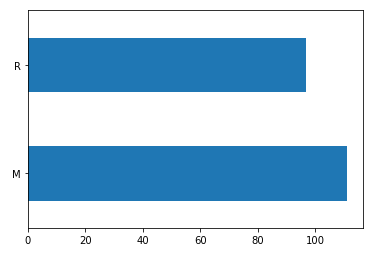
\includegraphics[width=0.3\textwidth]{imagenes/sonar-equilibrio.png}
    \end{center}

    donde existen $111$ datos para la clase Mina y $97$ datos para la clase 
    Roca. Como no hay mucha diferencia entre ambas clases, entonces no es 
    necesario rebalancear de alguna manera el conjunto de datos. 

    Aunque los metadatos dicen que todos los predictores van de $0$ a $1$, 
    todavía encontramos que hay varios de ellos que tienen valores relativamente
    menores en comparación con la mayoría. También encontramos que no hay
    ningún valor alto más grande que $1$.
    \begin{center}
        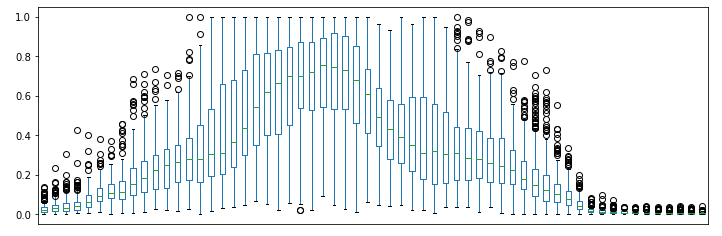
\includegraphics[width=0.5\textwidth]{imagenes/sonar-boxes.png}
    \end{center}

    La matriz de correlación nos indica que hay alguna estructura en el órden 
    de los atributos: el color rojo alrededor de la diagonal sugiere que los 
    atributos que están uno al lado del otro están más correlacionados entre 
    sí (es decir, cada variable tiene una gran correlación positiva con sus 
    vecinos), las manchas azules sugieren alguna correlación negativa moderada 
    entre los atributos que están más alejados unos de otros. Esto tiene 
    sentido si el órden de los atributos se refiere al ángulo de los sensores 
    para el chirrido del sonar.
    \begin{center}
        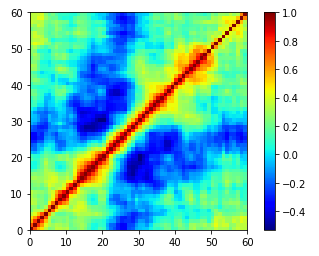
\includegraphics[width=0.25\textwidth]{imagenes/sonar-correlacion.png}
    \end{center}

    Ahora bien, para el procesamiento de datos separamos al conjunto de datos 
    en dos:
    \begin{itemize}
        \item $X$: el cual está conformado por las primeras $59$ columnas del 
        dataset original.
        \item $y$: el cual está conformado por la columna $60$ del dataset 
        original.
    \end{itemize}

    La gráfica de cajas nos sugiere que debemos estandarizar los datos de 
    entrada, por lo que usamos la clase \textbf{StandardScaler} para lograr 
    esto (recordándo que ésta elimina la media y escala los datos de forma que 
    su varianza sea igual a $1$). 

    La variable de salida (la columna $60$) es un string \textbf{M} o \textbf{R}.
    Debemos convertirlos en valores enteros entre $0$ y $1$, y para lograr esto 
    usamos la clase \textbf{LabelEncoder} (la cual modelará la codificación 
    requerida usando todo el conjunto de datos a traves de la función 
    \texttt{fit()} y luego aplicará la codificación para crear una nueva variable 
    de salida usando la función \texttt{transform()}).

    Para crear el modelo de regresión lineal, dividimos nuestro conjunto de datos 
    ya modificado en entrenamiento ($80\%$) y prueba ($20\%$). Luego, simplemente 
    creamos una instancia de \\ 
    \texttt{LogisticRegression}  y lo entrenamos.

    Los resultados obtenidos fueron los siguientes:
    \begin{center}
        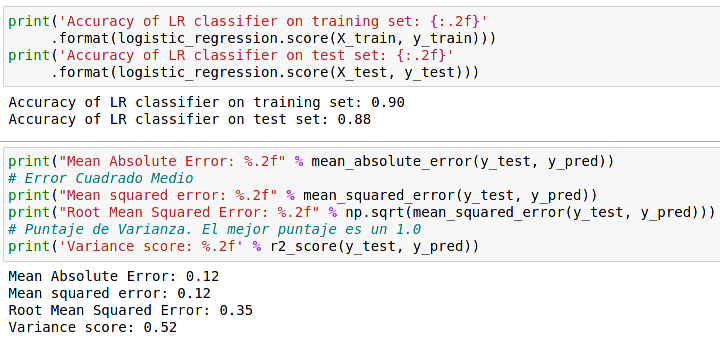
\includegraphics[width=0.8\textwidth]{imagenes/sonar-lg1.png}
        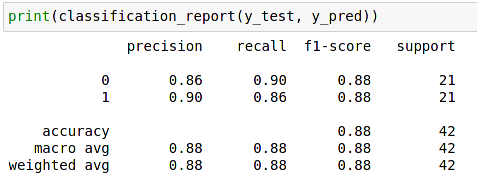
\includegraphics[width=0.5\textwidth]{imagenes/sonar-lg2.png}
    \end{center}

    donde en particular podemos notar que 
    \begin{itemize}
        \item Obtenemos un $90\%$ de precisión en el conjunto de entrenamiento 
        y un $88\%$ de precisión en el conjunto de prueba.

        \item Obtenemos MSE de $0.12$ (con un puntaje de varianza de $0.52$).

        \item Obtenemos $86\%$ de precisión para los datos correspondientes a 
        metales y $90\%$ de precisión para los datos correspondientes a las 
        rocas.
    \end{itemize}
    
    Por otro lado, usaremos PCA para obtener la lista de atributos que tienen 
    mayor varianza (mayor poder explicativo). Éstos serán los componentes 
    principales. Realizamos un par de gráficas para poder determinar el 
    número de estos componentes.
    \begin{figure}[ht]
        \centering
        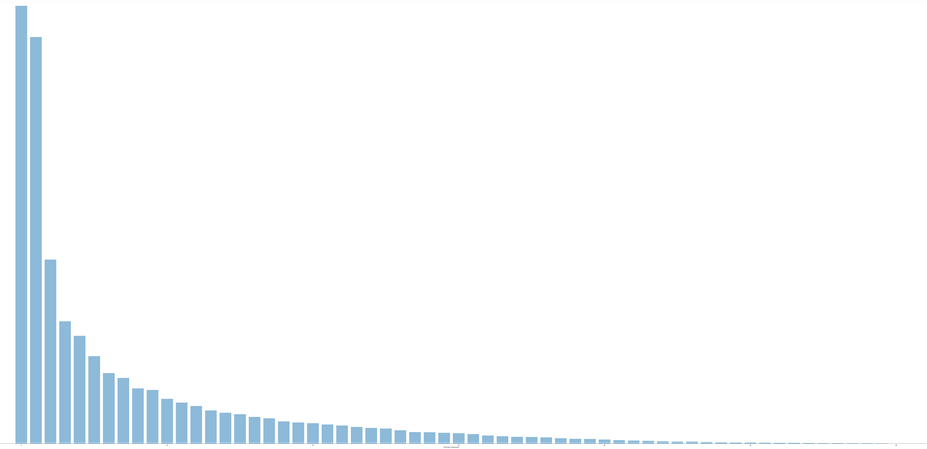
\includegraphics[width=0.7\textwidth]{imagenes/sonar-pca1.png}
        \caption{Variance Ratio vs Principal componentes }
    \end{figure}
    \begin{figure}[ht]
        \centering
        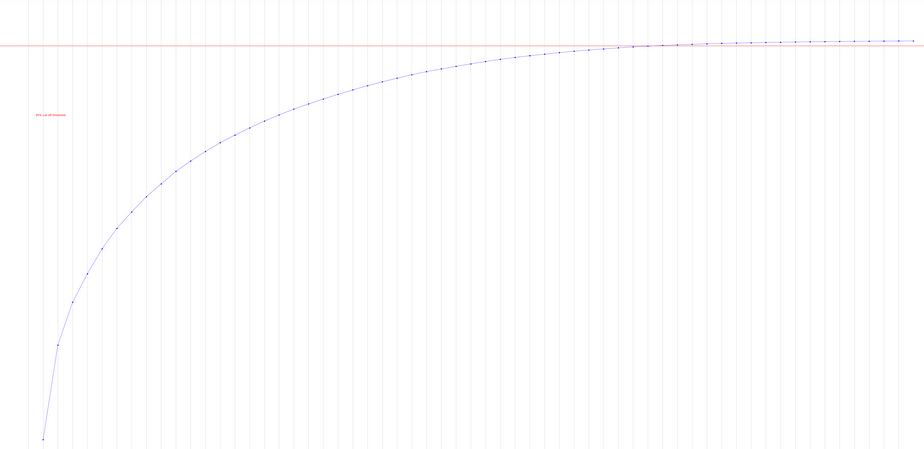
\includegraphics[width=0.8\textwidth]{imagenes/sonar-pca2.png}
        \caption{Cumulative variance vs Number of Components}
    \end{figure}


    Donde obtenemos que con $43$ componentes tenemos un $99\%$ de la 
    varianza explicada (queremos una v.e. entre $95\%$ y $99\%$, pero me ha 
    gustado más al resultado con este valor). Así, creamos una instancia 
    de PCA con un número de $43$ componentes principales y la entrenamos, 
    para después pasarle este nuevo conjunto $X\_pca$ al modelo de 
    \texttt{LogisticRegression} y entrenarlo.

    Los resultados obtenidos fueron los siguientes:
    \begin{center}
        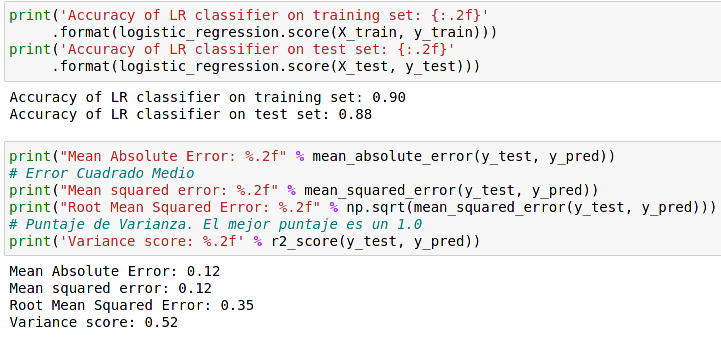
\includegraphics[width=0.8\textwidth]{imagenes/sonar-pca3.png}
        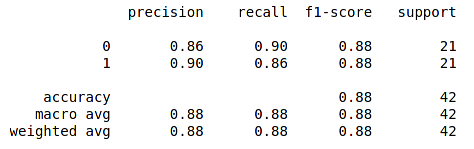
\includegraphics[width=0.5\textwidth]{imagenes/sonar-pca4.png}
    \end{center}

    donde en particular podemos notar que 
    \begin{itemize}
        \item Obtenemos un $90\%$ de precisión en el conjunto de entrenamiento 
        y un $88\%$ de precisión en el conjunto de prueba.

        \item Obtenemos MSE de $0.12$ (con un puntaje de varianza de $0.52$).

        \item Obtenemos $86\%$ de precisión para los datos correspondientes a 
        metales y $90\%$ de precisión para los datos correspondientes a las 
        rocas.
    \end{itemize}

    Así, podemos concluir que obtenemos la misma precisión que en el modelo 
    anterior usando $43$ componentes principales ($16$ columnas menos). Esto 
    puede ser causado por el nivel de correlación que notamos al analizar los 
    datos.

    % Ejercicio 3.
    \item Diseña un experimento para determinar para qué umbral es posible tener 
    un conjunto de datos no balanceado.

    % Ejercicio 4.
    \item Reproduce la gráfica de la información mutua del seno contra él mismo 
    considerándo un corrimiento de $50$ posiciones.

    % Ejercicio 5.
    \item El dataset de \texttt{seatbelt.csv} representa una serie de datos 
    temporales de diversos atributos que hacen referencia a la mortalidad 
    asociada a los accidentes de tránsito en Gran Bretaña en el periodo de 
    $1969$ y $1984$. La legislación para utilizar el cinturón de seguridad de 
    manera obligatoria fue introducida el $31$ de enero de $1983$. Ajusta un 
    modelo lineal generalizado para determinar la probabilidad de morir en 
    un accidente de tránsito y responde las siguientes preguntas:
    \begin{itemize}
        % Ejercicio 5.a
        \item ¿Volver obligatorio el cinturón de seguridad disminuyó la 
        probabilidad de morir en algún accidente de tránsito?

        % Ejercicio 5.b
        \item ¿Qué otra conclusión puedes generar a partir del modelo que 
        ajustaste? 
    \end{itemize}

    Se espera que lleves a cabo la normalización o estandarización del 
    dataset, la transformación de las variables que consideres pertinente y 
    que propongas qué variables tienen más o menos importancia en la 
    probabilidad de morir en un accidente de tránsito.
\end{enumerate}

\end{document}
